\documentclass[tikz]{standalone}
\usepackage{amsmath,amssymb}
\usepackage{graphicx}
\usepackage{xcolor}

\begin{document}
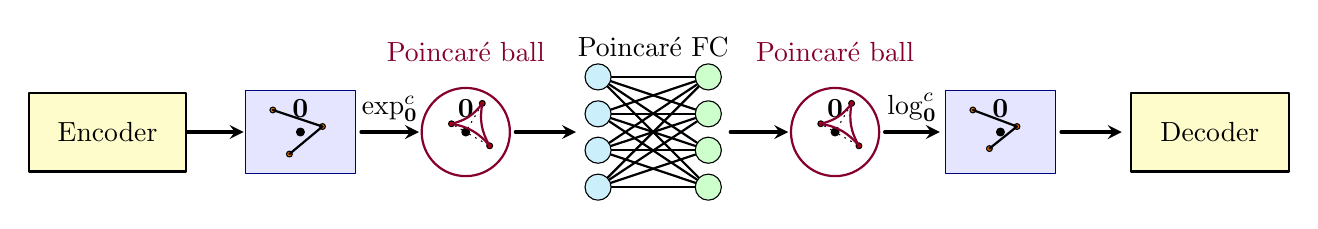
\begin{tikzpicture}[scale=0.7, >=stealth, line cap=round, line join=round]

%------------------------------------------------------------------
% 1) ENCODER SCOPE
%------------------------------------------------------------------
\begin{scope}[xshift=0.5cm]
  \node[draw=black, fill=yellow!20, thick,
        rectangle, minimum width=2.0cm, minimum height=1cm,
        align=center] (encoder) at (0,0) {Encoder};

  % Encoder's east coordinate (for the outgoing arrow)
  \coordinate (encoderEast) at (encoder.east);
\end{scope}
% Encoder east absolute: 0.5 + 1.1 = 1.6

%------------------------------------------------------------------
% 2) LEFT EUCLIDEAN PLANE SCOPE
%------------------------------------------------------------------
% Set xshift=3.6 so that the entry point becomes at 3.6 + (-0.2) = 3.4.
\begin{scope}[xshift=3.0cm]
  \coordinate (entryLeftPlane) at (-0.03,0);

  \path[fill=blue!10, draw=blue!50!black]
        (0,0.75) rectangle (2,-0.75);

  \coordinate (Oeuc) at (1,0);
  \node[draw=black,circle,fill=black,inner sep=1pt,
        label=above:$\mathbf{0}$] at (Oeuc) {};

  \coordinate (E1) at (0.5, 0.4);
  \coordinate (E2) at (0.8,-0.4);
  \coordinate (E3) at (1.4, 0.1);

  \foreach \pt in {E1,E2,E3} {
    \draw[fill=orange!90!black] (\pt) circle (1.5pt);
  }
  \draw[thick] (E1) -- (E3) -- (E2);

  % Define the east exit of the left Euclidean plane.
  \coordinate (leftPlaneEast) at (2.1,0);
\end{scope}
% leftPlaneEast absolute: 3.6+2.2 = 5.8

% Arrow from Encoder to Left Euclidean (length = 1.8 cm):
% From encoderEast at absolute x=1.6 to entryLeftPlane at 3.6-0.2=3.4.
\draw[->, very thick] (encoderEast) -- (entryLeftPlane);

%------------------------------------------------------------------
% 3) FIRST (OUTPUT) POINCARÉ ball SCOPE
%------------------------------------------------------------------
% We want the arrow from Left Euclidean to First ball to be 1.2 cm.
% leftPlaneEast is at 5.8, so First ball's entry should be at 5.8+1.2 = 7.0.
% Since First ball's entry is defined as (-1,0), set its xshift so that: xshift - 1 = 7.0, i.e. xshift = 8.0.
\begin{scope}[xshift=7.0cm]
  \coordinate (entryPoinc1) at (-0.85,0);

  \def\R{0.8}
  \draw[thick, purple!70!black] (0,0) circle (\R);

  \node[draw=black,circle,fill=black,inner sep=1pt,
        label=above:$\mathbf{0}$] (O1) at (0,0) {};

  \coordinate (P1) at ({0.6*cos(60)},{0.6*sin(60)});
  \coordinate (P2) at ({0.5*cos(-30)},{0.5*sin(-30)});
  \coordinate (P3) at ({0.3*cos(150)},{0.3*sin(150)});

  \foreach \pt in {P1,P2,P3} {
    \draw[fill=red!80!black] (\pt) circle (1.5pt);
  }

  \draw[dotted] (O1) -- (P1);
  \draw[dotted] (O1) -- (P2);
  \draw[dotted] (O1) -- (P3);

  \draw[thick, purple!70!black] (P1) to[bend right=20] (P2);
  \draw[thick, purple!70!black] (P2) to[bend right=20] (P3);
  \draw[thick, purple!70!black] (P3) to[bend right=20] (P1);

  \node[above, purple!70!black]
    at (0, {0.8+0.3})
    {Poincaré ball};

  % Define the east exit of the First ball.
  \coordinate (poinc1East) at (0.9,0);
\end{scope}
% First ball entry absolute: 8.0-1 = 7.0.
% First ball exit absolute: 8.0+1.3 = 9.3.

% Arrow from Left Euclidean to First ball (length = 1.2 cm):
% From leftPlaneEast at 5.8 to First ball entry at 7.0.
\draw[->, very thick] (leftPlaneEast) -- (entryPoinc1)
  node[midway,above] {$\exp_{\mathbf{0}}^{c}$};

%------------------------------------------------------------------
% 4) FULLY CONNECTED LAYER (FC) SCOPE
%------------------------------------------------------------------
% We want the arrow from First ball to FC to be 0.6 cm.
% First ball exit is at 9.3, so FC entry should be at 9.3+0.6 = 9.9.
% Since FC entry is defined as (-0.5,0), set FC's xshift so that: xshift - 0.5 = 9.9, i.e. xshift = 10.4.
\begin{scope}[xshift=9.4cm]
  \coordinate (entryFC) at (-0.4,0);

  % 4 input neurons
  \foreach \index/\y in {1/1, 2/0.33, 3/-0.33, 4/-1} {
    \node[draw=black, circle, fill=cyan!20, minimum size=6pt]
          (in\index) at (0,\y) {};
  }

  % 4 output neurons
  \foreach \index/\y in {1/1, 2/0.33, 3/-0.33, 4/-1} {
    \node[draw=black, circle, fill=green!20, minimum size=6pt]
          (out\index) at (2,\y) {};
  }

  % Connect them
  \foreach \i in {1,2,3,4} {
    \foreach \j in {1,2,3,4} {
      \draw[thick] (in\i) -- (out\j);
    }
  }

  \node[above] at (1,1.2) {Poincaré FC};

  % Define the east exit of the FC layer.
  \coordinate (fcEast) at (2.4,0);
\end{scope}
% FC entry absolute: 10.4-0.5 = 9.9.
% FC exit absolute: 10.4+2.5 = 12.9.

% Arrow from First ball to FC (length = 0.6 cm):
% From First ball exit at 9.3 to FC entry at 9.9.
\draw[->, very thick] (poinc1East) -- (entryFC);

%------------------------------------------------------------------
% 5) SECOND POINCARÉ ball SCOPE
%------------------------------------------------------------------
% We want the arrow from FC to Second ball to be 0.6 cm.
% FC exit is at 12.9, so Second ball entry should be at 12.9+0.6 = 13.5.
% Since Second ball entry is defined as (-1,0), set its xshift so that: xshift - 1 = 13.5, i.e. xshift = 14.5.
\begin{scope}[xshift=13.7cm]
  \coordinate (entryPoinc2) at (-0.85,0);

  \def\R{0.8}
  \draw[thick, purple!70!black] (0,0) circle (\R);
  \node[draw=black,circle,fill=black,inner sep=1pt,
        label=above:$\mathbf{0}$] (O2) at (0,0) {};

  % Points
  \coordinate (Q1) at ({0.6*cos(60)},{0.6*sin(60)});
  \coordinate (Q2) at ({0.5*cos(-30)},{0.5*sin(-30)});
  \coordinate (Q3) at ({0.3*cos(150)},{0.3*sin(150)});

  \foreach \pt in {Q1,Q2,Q3} {
    \draw[fill=red!80!black] (\pt) circle (1.5pt);
  }
  \draw[dotted] (O2) -- (Q1);
  \draw[dotted] (O2) -- (Q2);
  \draw[dotted] (O2) -- (Q3);

  \draw[thick, purple!70!black] (Q1) to[bend right=20] (Q2);
  \draw[thick, purple!70!black] (Q2) to[bend right=20] (Q3);
  \draw[thick, purple!70!black] (Q3) to[bend right=20] (Q1);

  \node[above, purple!70!black]
    at (0, {0.8 + 0.3})
    {Poincaré ball};

  % Define the east exit of the Second ball.
  \coordinate (poinc2East) at (0.9,0);
\end{scope}
% Second ball entry absolute: 14.5-1 = 13.5.
% Second ball exit absolute: 14.5+1.2 = 15.7.

% Arrow from FC to Second ball (length = 0.6 cm):
% From FC exit at 12.9 to Second ball entry at 13.5.
\draw[->, very thick] (fcEast) -- (entryPoinc2);

%------------------------------------------------------------------
% 6) RIGHT EUCLIDEAN PLANE SCOPE
%------------------------------------------------------------------
% We want the arrow from Second ball to Right Euclidean to be 1.2 cm.
% Second ball exit is at 15.7, so Right Euclidean entry should be at 15.7+1.2 = 16.9.
% Since Right Euclidean entry is defined as (-0.2,0), set its xshift so that: xshift - 0.2 = 16.9, i.e. xshift = 17.1.
\begin{scope}[xshift=15.7cm]
  \coordinate (entryRightEuc) at (-0.1,0);

  \path[fill=blue!10, draw=blue!50!black]
       (0,0.75) rectangle (2,-0.75);

  \coordinate (OeucRight) at (1,0);
  \node[draw=black,circle,fill=black,inner sep=1pt,
        label=above:$\mathbf{0}$] at (OeucRight) {};

  \coordinate (E4) at (0.5,0.4);
  \coordinate (E5) at (0.8,-0.3);
  \coordinate (E6) at (1.3,0.1);

  \foreach \pt in {E4,E5,E6} {
    \draw[fill=orange!90!black] (\pt) circle (1.5pt);
  }
  \draw[thick] (E4) -- (E6) -- (E5);

  % Define the east exit of the Right Euclidean plane.
  \coordinate (rightEucEast) at (2.1,0);
\end{scope}
% Right Euclidean entry absolute: 17.1-0.2 = 16.9.
% Right Euclidean exit absolute: 17.1+2.0 = 19.1.

% Arrow from Second ball to Right Euclidean (length = 1.2 cm):
% From Second ball exit at 15.7 to Right Euclidean entry at 16.9.
\draw[->, very thick] (poinc2East) -- (entryRightEuc)
  node[midway,above] {$\log_{\mathbf{0}}^{c}$};

%------------------------------------------------------------------
% 7) DECODER SCOPE
%------------------------------------------------------------------
% We want the arrow from Right Euclidean to Decoder to be 1.8 cm.
% Right Euclidean exit is at 19.1, so Decoder entry should be at 19.1+1.8 = 20.9.
% Since Decoder entry is defined as (-1.7,0), set its xshift so that: xshift - 1.7 = 20.9, i.e. xshift = 22.6.
\begin{scope}[xshift=20.5cm]
  \coordinate (entryDecoder) at (-1.6,0);

  \node[draw=black, fill=yellow!20, thick,
        rectangle, minimum width=2.0cm, minimum height=1cm,
        align=center] (decoder) at (0,0) {Decoder};
\end{scope}
% Decoder entry absolute: 22.6-1.7 = 20.9.

% Arrow from Right Euclidean to Decoder (length = 1.8 cm):
% From Right Euclidean exit at 19.1 to Decoder entry at 20.9.
\draw[->, very thick] (rightEucEast) -- (entryDecoder);

\end{tikzpicture}
\end{document}
